\part{Physique (13 points)}
\section{Applications de la radioactivité en médecine}
La radioactivité est utilisée dans plusieurs domaines comme la médecine ou l'on
peut diagnostiquer la maladie par imagerie médicale en utilisant des substances
radioactives comme le fluorodéoxyglucoce (en abrégé FDG) qui contient du fluor
radioactif \ce{_{9}^{18} F}.

Après avoir injecté le FDG par voie intraveineuse à un patient, on peut suivre
les rayonnements émis à l'aide d'une camera spéciale.

\begin{donnees}
    \begin{itemize}
        \item Énergie de liaison par nucléon~:\par
            \begin{table}[H]
              \flushright
              \renewcommand{\arraystretch}{1.6}
              \begin{tabularx}{0.94\textwidth}{|p{5cm}|C|C|C|C|}
                  \hline
                  \multicolumn{1}{|l|}{Noyau} & \ce{_{7}^{14}N} &
                  \ce{_{8}^{18}O} & \ce{_{9}^{18}F} & \ce{_{10}^{18}Ne} \\
                  \hline
                  \raisebox{0mm}[7mm][4mm]{$\frac{E_{L}}{A}$ (\unit{\MeV}/nucléon)} & 7,473 &
                  7,765 & 6,629 & 7,338 \\
                  \hline
              \end{tabularx}
             \end{table} 
        \item Demi vie du fluor \ce{_{9}^{18}F}~: $t_{1/2}=\qty{110}{\min}$.
    \end{itemize}
\end{donnees}

\begin{enumerate}
    \item \textbf{Désintégration du noyau de fluor \ce{_{9}^{18}F}}

          Le fluor \ce{_{9}^{18}F} est radioactif $\beta^{+}$.
          \begin{enumerate}
              \item Écrire l'équation de désintégration du fluor \ce{_{9}^{18}F}
                    en précisant le noyau fils.
              \item Recopier sur votre copie le numéro de la question et écrire la
                    lettre correspondante à la seule proposition vraie parmi~:
                    \begin{enumerate}
                        \item Le noyau de fluor \ce{_{9}^{18}F} est constitué de
                              18 neutrons et 9 protons.
                        \item La masse du noyau \ce{_{9}^{18}F} est inférieure à
                              la somme des masses de ses nucléons.
                        \item L'unité de l'énergie de liaison d'un noyau est le
                              (\unit{\MeV}/nucléon).
                        \item La constante radioactive s'exprime par la relation
                              $\lambda=t_{1/2} \cdot \ln 2$.
                    \end{enumerate}
              \item Déterminer, en justifiant votre réponse, le noyau le plus
                    stable parmi \ce{_{7}^{14}N}~; \ce{_{8}^{18}O}~;
                    \ce{_{10}^{18}Ne}.
          \end{enumerate}

    \item \textbf{Injection du FDG à un patient}

          Pour réaliser un examen d'imagerie médicale à un patient, on lui
          injecte une dose de FDG d'activité $a=\qty{5,0e8}{\Bq}$.

          La dose du FDG a été préparée dans le bloc de médecine nucléaire d'un
          hôpital à 5 heures du matin pour l'injecter au patient à 10 heures du
          même jour. L'activité du \ce{_{9}^{18}F} à 5 heures est $a_{0}$.

          Vérifier que $a_{0} \simeq \qty{3,3e9}{\Bq}$.
\end{enumerate}


\section*{Exercice 2 (5 points)~: Réponse d'un dipôle}
Un professeur désire déterminer expérimentalement la valeur de la capacité $C$
d'un condensateur. Pour cela il étudie la charge de ce condensateur par un
générateur idéal de courant et vérifie la valeur obtenue de la capacité par
l'étude de la réponse d'un dipôle $R C$ à un échelon de tension descendant, et
ce dans le but d'utiliser ce condensateur dans l'étude énergétique d'un circuit
$R L C$ série.

\subsection{Étude de la charge d'un condensateur par un générateur idéal du
courant}
Pour étudier la charge du condensateur, le professeur réalise le montage de la
Fig.~\ref{fig:svt_national_2016_normale_phys_ex2_1} constitué des éléments
suivants~:

\begin{itemize}
    \item un générateur idéal de courant qui alimente le circuit par un courant
          électrique d'intensité constante $I_{0}=\qty{2e-5}{\A}$~;
    \item un conducteur ohmique de résistance $R_{0}$~;
    \item un condensateur de capacité $C$~;
    \item un interrupteur $\mathrm{K}$.
\end{itemize}

À $t_{0}=0$, le professeur ferme l'interrupteur $\mathrm{K}$ et suit à l'aide
d'un dispositif convenable, les variations de la tension $u_{C}(t)$ aux bornes
du condensateur. La Fig.~\ref{fig:svt_national_2016_normale_phys_ex2_2}
représente la courbe obtenue.

\begin{minipage}{0.49\linewidth}
    \begin{figure}[H]
        \centering
        \raisebox{8mm}{%
        \begin{circuitikz}
            \newdimen\d \d=3cm
            \draw (0,0) coordinate (O)
                to[I,v^>=,name=I0] ++(0,\d)
                to[switch,l=$\mathrm{K}$] ++(\d,0)
                to[R,l=$R_{0}$] ++(\d,0)
                to[C,l_=$C$,v^<=$u_{C}$,i>^={ }] ++(0,-\d)
                to[short] (O);
            \fixedvlen{I0}{$I_{0}$}
        \end{circuitikz}}
        \caption{}
        \label{fig:svt_national_2016_normale_phys_ex2_1}
    \end{figure}
\end{minipage}
\begin{minipage}{0.49\linewidth}
\begin{figure}[H]
    \centering
    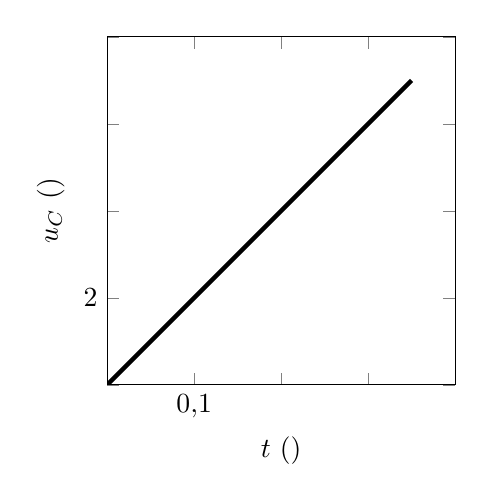
\begin{tikzpicture}[]
        \begin{axis}[
                width=6cm,height=6cm,
                xlabel=$t~(\unit{\s})$,ylabel=$u_{C}~(\unit{\V})$,
                xmin=0,xmax=0.4,
                ymin=0,ymax=8,
                variable=\t,
                domain=0:0.35,
                xticklabels={,,$0{,}1$,,},
                yticklabels={,,$2$,,},
            ]
            \addplot[ultra thick] {20*t};
        \end{axis}
    \end{tikzpicture}
    \caption{}
    \label{fig:svt_national_2016_normale_phys_ex2_2}
\end{figure}
\end{minipage}


\begin{enumerate}
    \item En exploitant la courbe, déterminer l'expression de la tension
          $u_{C}(t)$.
    \item \label{item:culcul_C}
          Montrer que $C=\qty{1}{\uF}$.
\end{enumerate}


\subsection{Étude de la réponse d'un dipôle $R C$ à un échelon de tension
descendant}
Pour s'assurer de la valeur de la capacité $C$ trouvée précédemment, le
professeur réalise le montage de la
Fig.~\ref{fig:svt_national_2016_normale_phys_ex2_3} constitué des éléments
suivants~:

\begin{itemize}
    \item un générateur idéal de tension de force électromotrice $E$~;
    \item un conducteur ohmique de résistance $R=\qty{2e3}{\ohm}$~;
    \item le condensateur précédent de capacité $C$~;
    \item un interrupteur $\mathrm{K}$ à double position.
\end{itemize}

Le professeur charge totalement le condensateur en plaçant l'interrupteur en
position~(1), et puis il le bascule en position~(2) à l'instant $t_{0}=0$. Il
suit à l'aide d'un dispositif convenable les variations de la tension $u_{c}(t)$
aux bornes du condensateur.
La Fig.~\ref{fig:svt_national_2016_normale_phys_ex2_4} représente la courbe
obtenue.



\begin{minipage}{0.49\linewidth}
    \begin{figure}[H]
        \centering
        \raisebox{1cm}{%
        \begin{circuitikz}
            \newdimen\d \d=3cm
            \node[cute spdt mid,rotate=90,label=below left:$\mathrm{K}$] (s) {};
            \draw (s.out 1) node[above] {$(1)$}
                to[short] ++(-0.7\d,0)
                to[vsource,v_<=$E$] ++(0,-\d) coordinate (tmp)
                to[short] (tmp -| s.in) coordinate (tmp)
                to[C,l=$C$,v=$u_{C}$,i^<=$i$] (s.in);
            \draw (s.out 2) node[above] {$(2)$}
                to[short] ++(0.7\d,0)
                to[R,l=$R$] ++(0,-\d)
                to[short] (tmp);
        \end{circuitikz}}
        \caption{}
        \label{fig:svt_national_2016_normale_phys_ex2_3}
    \end{figure}
\end{minipage}
\hfill
\begin{minipage}{0.49\linewidth}
\begin{figure}[H]
    \centering
    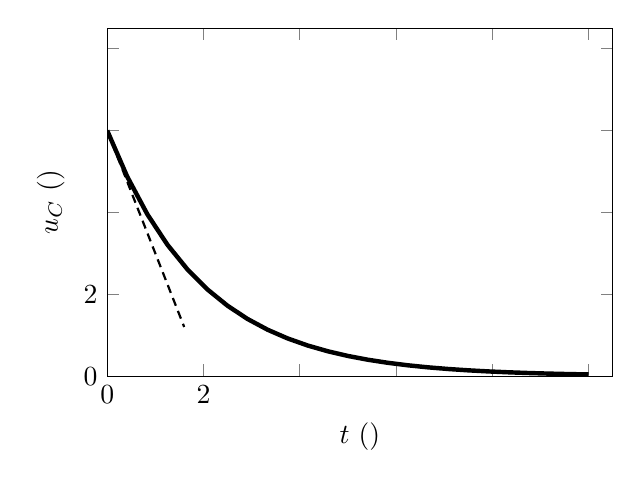
\begin{tikzpicture}[]
        \begin{axis}[
                width=8cm,height=6cm,
                xlabel=$t~(\unit{\ms})$,ylabel=$u_{C}~(\unit{\V})$,
                xmin=0,xmax=10.5,
                ymin=0,ymax=8.5,
                variable=\t,
                xtick distance=2,
                ytick distance=2,
                xticklabels={,$0$,$2$,,},
                yticklabels={,$0$,$2$,,},
            ]
            \addplot[ultra thick,domain=0:10] {6*exp(-t/2)};
            \addplot[thick,densely dashed,domain=0:1.6] {-3*t+6)};
        \end{axis}
    \end{tikzpicture}
    \caption{}
    \label{fig:svt_national_2016_normale_phys_ex2_4}
\end{figure}
\end{minipage}


\begin{enumerate}
    \item Établir l'équation différentielle vérifiée par la tension $u_{C}(t)$
          au cours de la décharge du condensateur.
    \item La solution de cette équation différentielle est de la forme
          $u_{C}(t)=A\times e^{-\frac{t}{\tau}}$. Déterminer les expressions de
          A et $\tau$ en fonction des paramètres du circuit.
    \item Déterminer graphiquement la valeur de $\tau$. Vérifier la valeur de
          $C$ trouvée dans la question~\ref{item:culcul_C}.
\end{enumerate}



\subsection{Étude énergétique du circuit RLC série}
Le professeur insère dans le montage de la
Fig.~\ref{fig:svt_national_2016_normale_phys_ex2_3}, en série avec le
conducteur ohmique, une bobine d'inductance $L=\qty{0.1}{\H}$ et de résistance
négligeable.

Après avoir chargé de nouveau et totalement le condensateur, le professeur
bascule l'interrupteur en position~(2), à l'instant $t_{0}=0$.
La Fig.~\ref{fig:svt_national_2016_normale_phys_ex2_5} représente les variations
de la tension $u_{c}(t)$ aux bornes du condensateur et de la tension $u_{R}(t)$
aux bornes du conducteur ohmique.

\begin{figure}[H]
    \centering
    \includegraphics[width=.7\textwidth]{2025_03_17_d0909ada06865003c630g-5(2)}
    \caption{}
    \label{fig:svt_national_2016_normale_phys_ex2_5}
\end{figure}
\begin{enumerate}
    \item Montrer que l'expression de l'énergie totale du circuit à un instant
          $t$ s'écrit~:
          \[
              \mathcal{E}=\frac{1}{2}C\times u_{C}^{2}+
              \frac{1}{2}\frac{L}{R^{2}}\times u_{R}^{2}
          \]
    \item Déterminer la valeur de
          $\Delta\mathcal{E}=\mathcal{E}_{1}-\mathcal{E}_{0}$, la variation de
          l'énergie totale du circuit entre les instants $t_{0}=0$ et
          $t_{1}=\qty{3.5}{\ms}$. Interpréter ce résultat.
\end{enumerate}



\section{Mouvement d'un solide soumis à des forces (constantes~-~variables)}
Les mouvements des solides dépendent des types de forces qui leurs sont
appliquées et des conditions initiales. L'étude de ces mouvements permet de
suivre l'évolution temporelle de certaines grandeurs physiques qui les
caractérisent.

Le but de cet exercice est l'étude du mouvement du centre d'inertie $G$ d'un
solide $\mathrm{(S)}$ dans le champ de pesanteur uniforme, et l'étude du
mouvement d'un système oscillant \{solide $\mathrm{(S)}$~-~ressort\} avec
détermination de certains paramètres qui caractérisent chaque mouvement.

\subsection{Étude du mouvement d'un solide dans le champ de pesanteur uniforme}
\begin{minipage}{0.64\linewidth}
    On lance, à un instant $t_{0}=0$ avec une vitesse initiale $\vec{v}_{0}$
    horizontale, un solide $\mathrm{(S)}$ de petites dimensions, de masse $m$,
    d'un point $A$ qui se trouve à la hauteur $h$ du sol. Le solide
    $\mathrm{(S)}$ tombe sur le sol au point d'impact $I$
    (Fig.~\ref{fig:2bac_svt_national_2016_normale_phys_ex3_1}).
    
    On étudie le mouvement du centre d'inertie $G$ dans le repère $(O,\ex,\ey)$
    lié à la terre supposé galiléen.
    \begin{donnees}
        \begin{itemize}
          \item Tous les frottements sont négligeables~;
          \item $g=\qty{9,8}{\a}$~; $h=OA=\qty{1}{\meter}$.
        \end{itemize}
    \end{donnees}
\end{minipage}
\hfill
\begin{minipage}{0.35\linewidth}
    \begin{figure}[H]
        \centering
        % \begin{tikzpicture}[thick]
        %     \def\g{9.8}
        %     \def\al{0}
        %     \pgfmathparse{-\g/(2*\vo^2*(cos(\al))^2)}\let\a=\pgfmathresult
        %     \begin{axis}[
        %             cycle list name=my color list,
        %             width=10cm,height=8cm,
        %             xlabel=$x$,ylabel=$y$,
        %             xmin=0,xmax=1,
        %             ymin=0,ymax=1,
        %             xtick={},
        %             xticklabels={},
        %             ytick={},
        %             yticklabels={},
        %         ]
        %         \addplot {};
        %     \end{axis}
        % \end{tikzpicture}
        \begin{tikzpicture}[thick]
            \def\xm{5}
            \def\ym{3.5}
            \def\h{2.3}
            \def\vo{18}
            \def\g{9.8}
            \pgfmathparse{-\g^2/(2*\vo^2)}\let\a=\pgfmathresult
            \pgfmathparse{sqrt(2*\h)*\vo/\g)}\let\xI=\pgfmathresult
            \draw[Latex-Latex]
                (0,\ym) node[below left,inner ysep=0pt] {$y$} |-
                (\xm,0) node[below left,inner xsep=0pt] {$x$};
            \draw[<->,very thick]
                (0,1) node[below left,inner ysep=0pt] {$\ey$} |-
                (1,0) node[below left,inner xsep=0pt] {$\ex$};
            \draw[domain=0:\xI] (0,\h) node[left] {$A$} plot(\x,{\a*\x^2+\h})
                node[below] {$I$};
            \draw[->,very thick]
                (0,\h) -- +(1.5,0) node[above left] {$\vec{v}_{0}$};
        \end{tikzpicture}
        \caption{}
        \label{fig:2bac_svt_national_2016_normale_phys_ex3_1}
    \end{figure}
\end{minipage}
\begin{enumerate}
    \item En appliquant la deuxième loi de Newton, établir les expressions
          littérales des équations horaires $x(t)$ et $y(t)$ du mouvement de
          $G$.
    \item En déduire l'expression littérale de l'équation de la trajectoire du
          mouvement de $G$.
    \item Calculer la valeur de $t_{I}$, l'instant d'arrivé de $\mathrm{(S)}$ au
          sol en $I$.
    \item On lance de nouveau, à un instant $t_{0}=0$, le solide $(S)$ du point
          $A$ avec une vitesse initiale
          $\vec{v}_{0}^{\prime}=3\cdot\vec{v}_{0}$.

          Recopier sur votre copie le numéro de la question et écrire la lettre
          correspondante à la seule proposition vraie~: \\
          la valeur de l'instant d'arrivé de $\mathrm{(S)}$ au sol vaut~: 

          \begin{tcbitemize}[raster columns=8,raster rows=1,
                  raster equal height=rows,
                  raster column skip=-0.8pt,raster force size=false,
                  raster every box/.style={valign=center},
                  label/.style={add to width=-1.4cm,halign=center},
                  answer/.style={add to width=1.4cm}]
              \tcbitem[label] $\mathrm{a}$
              \tcbitem[answer] $t^{\prime}=\qty{0.25}{\s}$
              \tcbitem[label] $\mathrm{b}$
              \tcbitem[answer] $t^{\prime}=\qty{0.35}{\s}$
              \tcbitem[label] $\mathrm{c}$
              \tcbitem[answer] $t^{\prime}=\qty{0.45}{\s}$
              \tcbitem[label] $\mathrm{d}$
              \tcbitem[answer] $t^{\prime}=\qty{0.65}{\s}$ 
          \end{tcbitemize}
\end{enumerate}



\subsection{Étude du mouvement d'un système oscillant \{solide (S)-ressort\}}
\begin{minipage}{0.65\linewidth}
    On fixe le solide $\mathrm{(S)}$ précédent à un ressort horizontal à spires
    non jointives, de masse négligeable et de constante de raideur $K$.
    
    À l'équilibre, le centre d'inertie $G$ coïncide avec l'origine du repère
    $(O,\ex)$ lié à la terre considéré comme galiléen
    (Fig.~\ref{fig:solide_ressort}).
    
    On écarte le solide $\mathrm{(S)}$ de sa position d'équilibre et on le
    libère sans vitesse initiale à l'instant $t_{0}=0$.
\end{minipage}
\hfill
\begin{minipage}{0.33\linewidth}
    \begin{figure}[H]
        \centering
        \begin{tikzpicture}
    \node[inner sep=0pt,minimum width=4.5cm,minimum height=3mm,
        top color=black!70] (sol) {};
    % Axe xx'
    \coordinate (O) at ($(sol.south west)!.8!(sol.south east)$);
    \draw[-Latex] (sol.south west)
        node[below right,inner xsep=0pt] {$x^{\prime}$} -- (O)
        node[below=0.4mm] {$O$} -- (sol.south east) -- ++(0.7,0)
        node[below left,inner xsep=0pt,inner ysep=2mm] {$x$};
    % Fixed
    \node[inner sep=0pt,draw,minimum width=3mm,minimum height=7mm,
        anchor=south,pattern=north west lines,
        thick] (fix) at ([xshift=3mm,yshift=0.4pt]sol.north west) {};
    % Solide (S)
    \node[inner sep=0pt,draw,minimum width=7mm,minimum height=7mm,
        anchor=south,rounded corners=2pt,thick,label=$\mathrm{(S)}$,
        fill=lightgray] (S) at
        ([yshift=0.4pt]O |- sol.north) {};
        %([xshift=-6mm,yshift=0.4pt]sol.north east) {};
    \node[inner sep=1pt,circle,fill,
        label={[right=-0.8mm,font=\scriptsize]:$G$}] (G) at (S.center) {};
    \draw[{Rectangle[length=1pt,width=4pt]}-{Stealth[length=5pt]},
        thick] (O) -- ++(0.8,0)
        node[below left,inner xsep=0pt] {$\ex$};
    % Ressort
    \draw[decoration={
          coil,
          aspect=0.3,
          segment length=2.0mm,
          amplitude=2.4mm,
          pre length=1mm,
          post length=1mm},
          decorate,thick,black] (fix.east) -- (S.west);
\end{tikzpicture}

        \caption{}
        \label{fig:solide_ressort}
    \end{figure}
\end{minipage}

\begin{donnees}
    \begin{itemize}
      \item Tous les frottements sont négligeables~;
      \item On choisit l'état où le ressort n'est pas déformé comme référence de
            l'énergie potentielle élastique $E_{pe}$ et le plan horizontal
            contenant $G$ comme état de référence de l'énergie potentielle de
            pesanteur $E_{pp}$.
    \end{itemize}
\end{donnees}
\begin{minipage}[t][][t]{0.68\linewidth}
    La courbe de la Fig.~\ref{fig:2bac_svt_national_2016_normale_phys_ex3_3}
    représente les variations de $E_{pe}$ en fonction de $x^{2}$, carré de
    l'abscisse $x$ du centre d'inertie $G$ dans le repère $(O,\ex)$.
    \begin{enumerate}
        \item En exploitant la courbe de la figure~(\ref{fig:Epe_de_x2}),
              trouver les valeurs de~:
              \begin{enumerate}
                  \item la constante de raideur $K$.
                  \item l'énergie potentielle élastique maximale $E_{pe,\max}$.
                  \item l'amplitude $X_{m}$ des oscillations.
              \end{enumerate}
        \item Déduire, en justifiant votre réponse, la valeur de l'énergie
              mécanique $E_{m}$ du système oscillant.
    \end{enumerate}
\end{minipage}
\hfill
\begin{minipage}[t][][t]{0.31\linewidth}
    \begin{figure}[H]
        \centering
        \begin{tikzpicture}
            \def\K{1}
            \begin{axis}[
                    xmin=0,xmax=19,
                    ymin=0,ymax=9.8,
                    width=6.5cm,height=6.5cm,
                    xlabel=$x^{2}~(\times\qty{1e-4}{\square\meter})$,
                    ylabel=$E_{pe}~(\unit{\mJ})$,
                    scaled ticks=false,
                    xtick distance=4, ytick distance=2,
                    xticklabels={,,4}, yticklabels={,,2},
                ]
                \addplot[domain=0:16,samples=200,
                    very thick,blue] {0.5*\K*x}
                    coordinate[pos=1](A);
            \end{axis}
            \draw[very thick,blue] ([yshift=-5mm]A) -- ([yshift=5mm]A);
            \foreach \f in {0.02,0.14,...,1}
                \draw[very thick,blue]
                    ($([yshift=-5mm]A)!\f!([yshift=5mm]A)$) -- ++(20:.2);
        \end{tikzpicture}
        \caption{}
        \label{fig:2bac_svt_national_2016_normale_phys_ex3_3}
    \end{figure}
\end{minipage}
\begin{enumerate}
    \setcounter{enumi}{2}
    \item Le centre d'inertie $G$ passe par la position d'équilibre dans le sens
          positif avec la vitesse $v=\qty{0,25}{\v}$.

          Montrer que l'expression de la période propre des oscillations s'écrit
          $T_{0}=2\pi\cdot\frac{X_{m}}{v}$. Calculer $T_{0}$.
\end{enumerate}



